\documentclass{article}
\usepackage[version=3]{mhchem}
\usepackage{graphicx}
\usepackage{csvsimple}
\usepackage{longtable}

\title{%
	MATH 376: Numerical Analysis \\
	\large  Project 1: Greenhouse gases and rainwater
	}
\author{Quan Vu}
\date{\today}

\begin{document}
	\maketitle
	
	\section{Abstract}
	This project aims at examining the relationship between the steady 	rise in atmospheric levels of several greenhouse gases and the pH of rainwater within the coressponding areas. In particular, this project looks at the annual levels of atmospheric carbon dioxide (\ce{CO2}) from the year 1959 to 2016 in Mauna Loa, Hawaiii. By computing the pH of water using the given data, it can be shown that the pH of rainwater has decreased from 5.63 to 5.58 over the years, and the trend shows that the pH level will likely drop lower.
	
	\section{Introduction}
	
	\subsection{Background information}
	It is well documented that the atmospheric levels of several “greenhouse” gases have been increasing over the past 57 years. It is also know that within areas with generally low human activities, carbon dioxide is the primary determinant of the pH of rainwater.
	
	\subsection{Problem description}
	This project aims at using the existing data regarding the levels of atmospheric \ce{CO2} around Mauna Loa to calculate the pH of rainwater in the same region over the years. This can be done with the help of five equations governing the chemistry of rainwater:
	\[ K_1 = \frac{10^6[H^+][HCO_3^-]}{K_HCO_2} \tag{1} \]
	\[ K_2 = \frac{[H^+][CO_3^{-2}]}{[HCO_3^-]} \tag{2} \]
	\[ K_\omega = [H^+][OH^-] \tag{3} \]
	\[ c_T = \frac{K_HCO_2}{10^6} + [HCO_3^-] + [CO_3^{-2}] \tag{4} \]
	\[ 0 = [HCO_3^-] + 2[CO_3^{-2}] + [OH^-] - [H^+] \tag{5} \]
	where ${K_H}$ is Henry's constant, ${K_1}$, ${K_2}$ and ${K_\omega}$ are equilibrium coefficients. The five unknowns are ${c_T}$ = total inorganic carbon, ${HCO_3^-}$ = bicarbonate, ${[CO_3^{-2}]}$ = carbonate, ${[H^+]}$ = hydrogen ion, ${[OH^-]}$ = hydroxyl ion.
	One major assumption with this approach is that we fix \ce{CO2} as the sole factor contributing to the pH of rainwater. In reality, many other greenhouse gases can also contribute to the fluctuation of pH.

	\subsection{Outline}
	Given the values ${K_H  = 10^{-1.46}}$, ${ K_1 =  10^{-6.3}}$, ${ K_2 = 10^{-10.3}}$, ${ K_\omega = 10^{-14}}$ and the annual \ce{CO2}, we can reduce equation (5) to be one that is in terms of ${[H^+]}$. We can compute ${[H^+]}$ and calculate the pH of rainwater using the equation:
	\[ pH = -log_{10}[H^+] \tag{6} \]
	
	\section{Numerical method}
	Firstly we convert the given equations so that the unknowns in (5) can be expressed in terms of ${[H^+]}$. \\
	From (1):
	\[ [HCO_3^-] = \frac{K_HK_1CO_2}{10^6[H^+]} \tag{1a} \] \\
	From (2) and from (1a):
	\[ [CO_3^{-2}] = \frac{K_2[HCO_3^-]}{[H^+]} \tag{2a} = \frac{K_HK_1K_2CO_2}{10^6[H^+]^2} \] \\
	From (3):
	\[ [OH^-] = \frac{K_\omega}{[H^+]} \tag{3a} \] \\
	From (4), (2a) and (3a):
	\[ c_T = \frac{K_HCO_2}{10^6} + \frac{K_HK_1CO_2}{10^6[H^+]} + \frac{K_HK_1K_2CO_2}{10^6[H^+]^2} \tag{4a} \]
	From 5, and from (1a), (2a), (3a):
	\[ 0 =  \frac{K_HK_1CO_2 + 10^6K_\omega}{10^6[H^+]} + \frac{2K_HK_1K_2CO_2}{10^6[H^+]^2}] - [H^+] \tag{5a} \]
	By using the bisection method on the above equation, we can find ${[H^+]}$.
	
	\section{Results}
	Using the methodology discussed above, we obtain the following results of the pH levels in rainwater in Mauna Loa, from 1959 to 2016:\\
	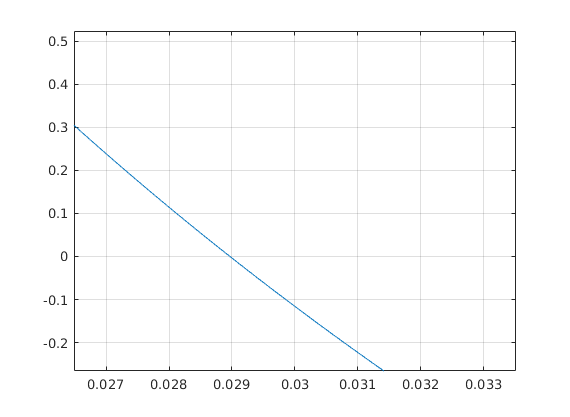
\includegraphics[scale=0.6]{untitled.jpg} \\
	For detailed results, consult the csv file in the project directory.
	
	\section{Discussion}
	From the calculations taken, the pH in the year 1959 was 5.63, and the pH calculated in 2016 was 5.58. While the decline seems small, we must keep in mind that pH is calculated by taking ${log_{10}}{[H^+]}$. This means that the concentration of Hydrogen ions in rainwater has increased over the year, and the trend does not seem to be stopping. In fact this trend can be modeled using the polyfit function in Matlab to give:
	\[pH = -5.523 \times 10^{-6}t^2 + 0.02101t - 14.33\] 
	where t denotes the year. If the trend continues, the pH of rainwater will drop below the threshold of 5.0, creating acid rain.
	\newpage
	\section{Bibliography}
	Data for annual atmospheric levels of \ce{CO2} are taken from: \\
	https://www.esrl.noaa.gov/gmd/ccgg/trends/data.html
\end{document}